% !TeX spellcheck = en_US
\documentclass[parskip=full]{report}

\usepackage{amsmath}
\usepackage{listings}
%\usepackage{beramono}
\usepackage{float}
\usepackage[utf8]{inputenc}
\usepackage[T1]{fontenc}
\usepackage{xcolor}
\usepackage[a4paper, margin={3cm}]{geometry}
\usepackage{hyperref}
\usepackage{graphicx}
\usepackage{svg}
\usepackage{subcaption}
\usepackage{float}
\usepackage{pdfpages}
\usepackage{array}

\usepackage{hyphenat}
\usepackage[english]{babel}
% Carattere monospaziato di default
\renewcommand{\ttdefault}{pcr}

\lstset{
	% wrap long lines on new line
	postbreak=\mbox{\textcolor{red}{$\hookrightarrow$}\space},
	breaklines=true, 
	columns=fullflexible,
	% tab and fonts
	tabsize=2,
	basicstyle=\ttfamily\small,
	% theme
	numbers=left,
	rulecolor=\color{black!30},	
	% UTF8 and escape
	escapeinside={\%TEX}{\^^M},
	inputencoding=utf8,
	extendedchars=true,
	literate={á}{{\'a}}1 {à}{{\`a}}1 {é}{{\'e}}1 {è}{{\`e}}1,
}


% Title Page
\title{
	
\includegraphics[width=0.333\textwidth]{assets/unipi1.png} \\
	\textsc{University of Pisa} \\
	\vspace{.5cm}
	Artificial Intelligence and Data Engineering \\
	Multimedia Information Retrieval and Computer Vision \\
	\vspace{2cm}
	{\huge \textsc{Search Engine ++} 
		\\IR system \& Index implementation}
}

\author{
	\begin{tabular}{lr}
		Dario Pagani & 585281 \\
		Franceso Londretti & 597086 \\
		Ricky Marinsalda & 585094
	\end{tabular}
}


\begin{document}
\maketitle
\tableofcontents


\chapter{Architecture}

\section{Tokenization}

\subsection{Logic}

\paragraph{UTF-8} 
The MSMARCO corpus contains several wrongly encoded documents, it seems their \textit{spider} wrongly interpreted certain documents as encoded in \texttt{latin1} --- a eight bit ASCII extension used by old Microsoft's software --- instead of \texttt{UTF-8} and then converted them in \texttt{UTF-8} interpreting their bytes as \texttt{UTF-8} data. To solve this issue we wrote a simple heuristic that tries to detect strange Unicode's entry-points that are likely the result of the processes; and a reverse encoding procedure that converts them back in their original \texttt{UTF-8} form. We didn't perform experiments so we cannot tell if this actually improves accuracy on the testing corpus.

\paragraph{Punctuation and splitting}
Our implementation takes a very simplistic approach to punctuation handling, that is all known western punctuation is removed and replaced with spaces, you can see the punctuation handled by the program in the source file \texttt{normalizer/PunctuationRemover.cpp}.

Words, that are tokens, are generated by splitting the resulting text by spaces.

\paragraph{Lower case}
Changing case of a Unicode word is a non trivial task and there are no fast ready-to-use libraries that directly operate on \texttt{UTF-8} --- instead they require a conversion to \texttt{UTF-16} or \texttt{UTF-32}, that we'd rather avoid, --- nevertheless we decided not to limit ourselves to only handle the case of ASCII's latin letters but we convert the case of \textit{latin1}'s latin letters --- that is a larger subset of Unicode latin letters. In conclusion all words written in latin characters are converted in lower-case.

\paragraph{Stemming}
Stemming is done using the Porter algorithm.

\subsection{Libraries}

\paragraph{Punctuation}
To replace punctuation with spaces we make use of regex expressions and run them on Hyperscan (or Vectorscan on non amd64 platforms), that is a fast regex engine that make use of SIMD instructions --- such as AVX-512 --- to speed up their solution.

\paragraph{Stemming}
To stem words, we make of the famous Snowball's stemmer implementation.

\section{Indices' organization}

\paragraph{}
We've designed the system to partition by document TODO TODO

\section{Indices}

bruh

\section{Lexica}

Since we're partitioning the dataset by document, to improve its parallelizability we make use of a local lexicon for each partition as well as a global lexicon used to store shared information.

\subsection{Disk Map}

To store the lexica it is necessary to use a disk-based data structure that
allows the program to quickly and efficiently seek the datum associated to a
particular key, that is an index term. To achieve this we make use of following:

\begin{itemize}
	\item to reduce disk seek time, the terms' data are compressed with
	\textit{integer compression} and the terms themselves with \textit{prefix compression}
	
	\item to minimize disk accesses, the terms are ordered lexicographically
	and partitioned in pages of the same size of the disk's page
	
	\item terms at the beginning of each page are stored in a separated array that fits in system memory, to quickly locate --- through \textit{binary search} or a \textit{trie visit} --- in which page a given term is located
\end{itemize}

\paragraph{Structure}
Let us call $|B|$ the size of a disk page, $|T|$ the maximum length off all terms stored, $m$ the maximum number of key-value pairs stored in a page, $k$ the number of pages used to store them all, $s_1 > s_2 > s_3 > \dots$ the terms to store and $d_1, d_2, d_3, \dots$ their data; and $s_{b_1} > s_{b_2} > \dots > s_{b_k}$ the terms that appear at the start of each page.

The following picture shows how our data are organized at high level

\begin{figure}[H]
	\centering
	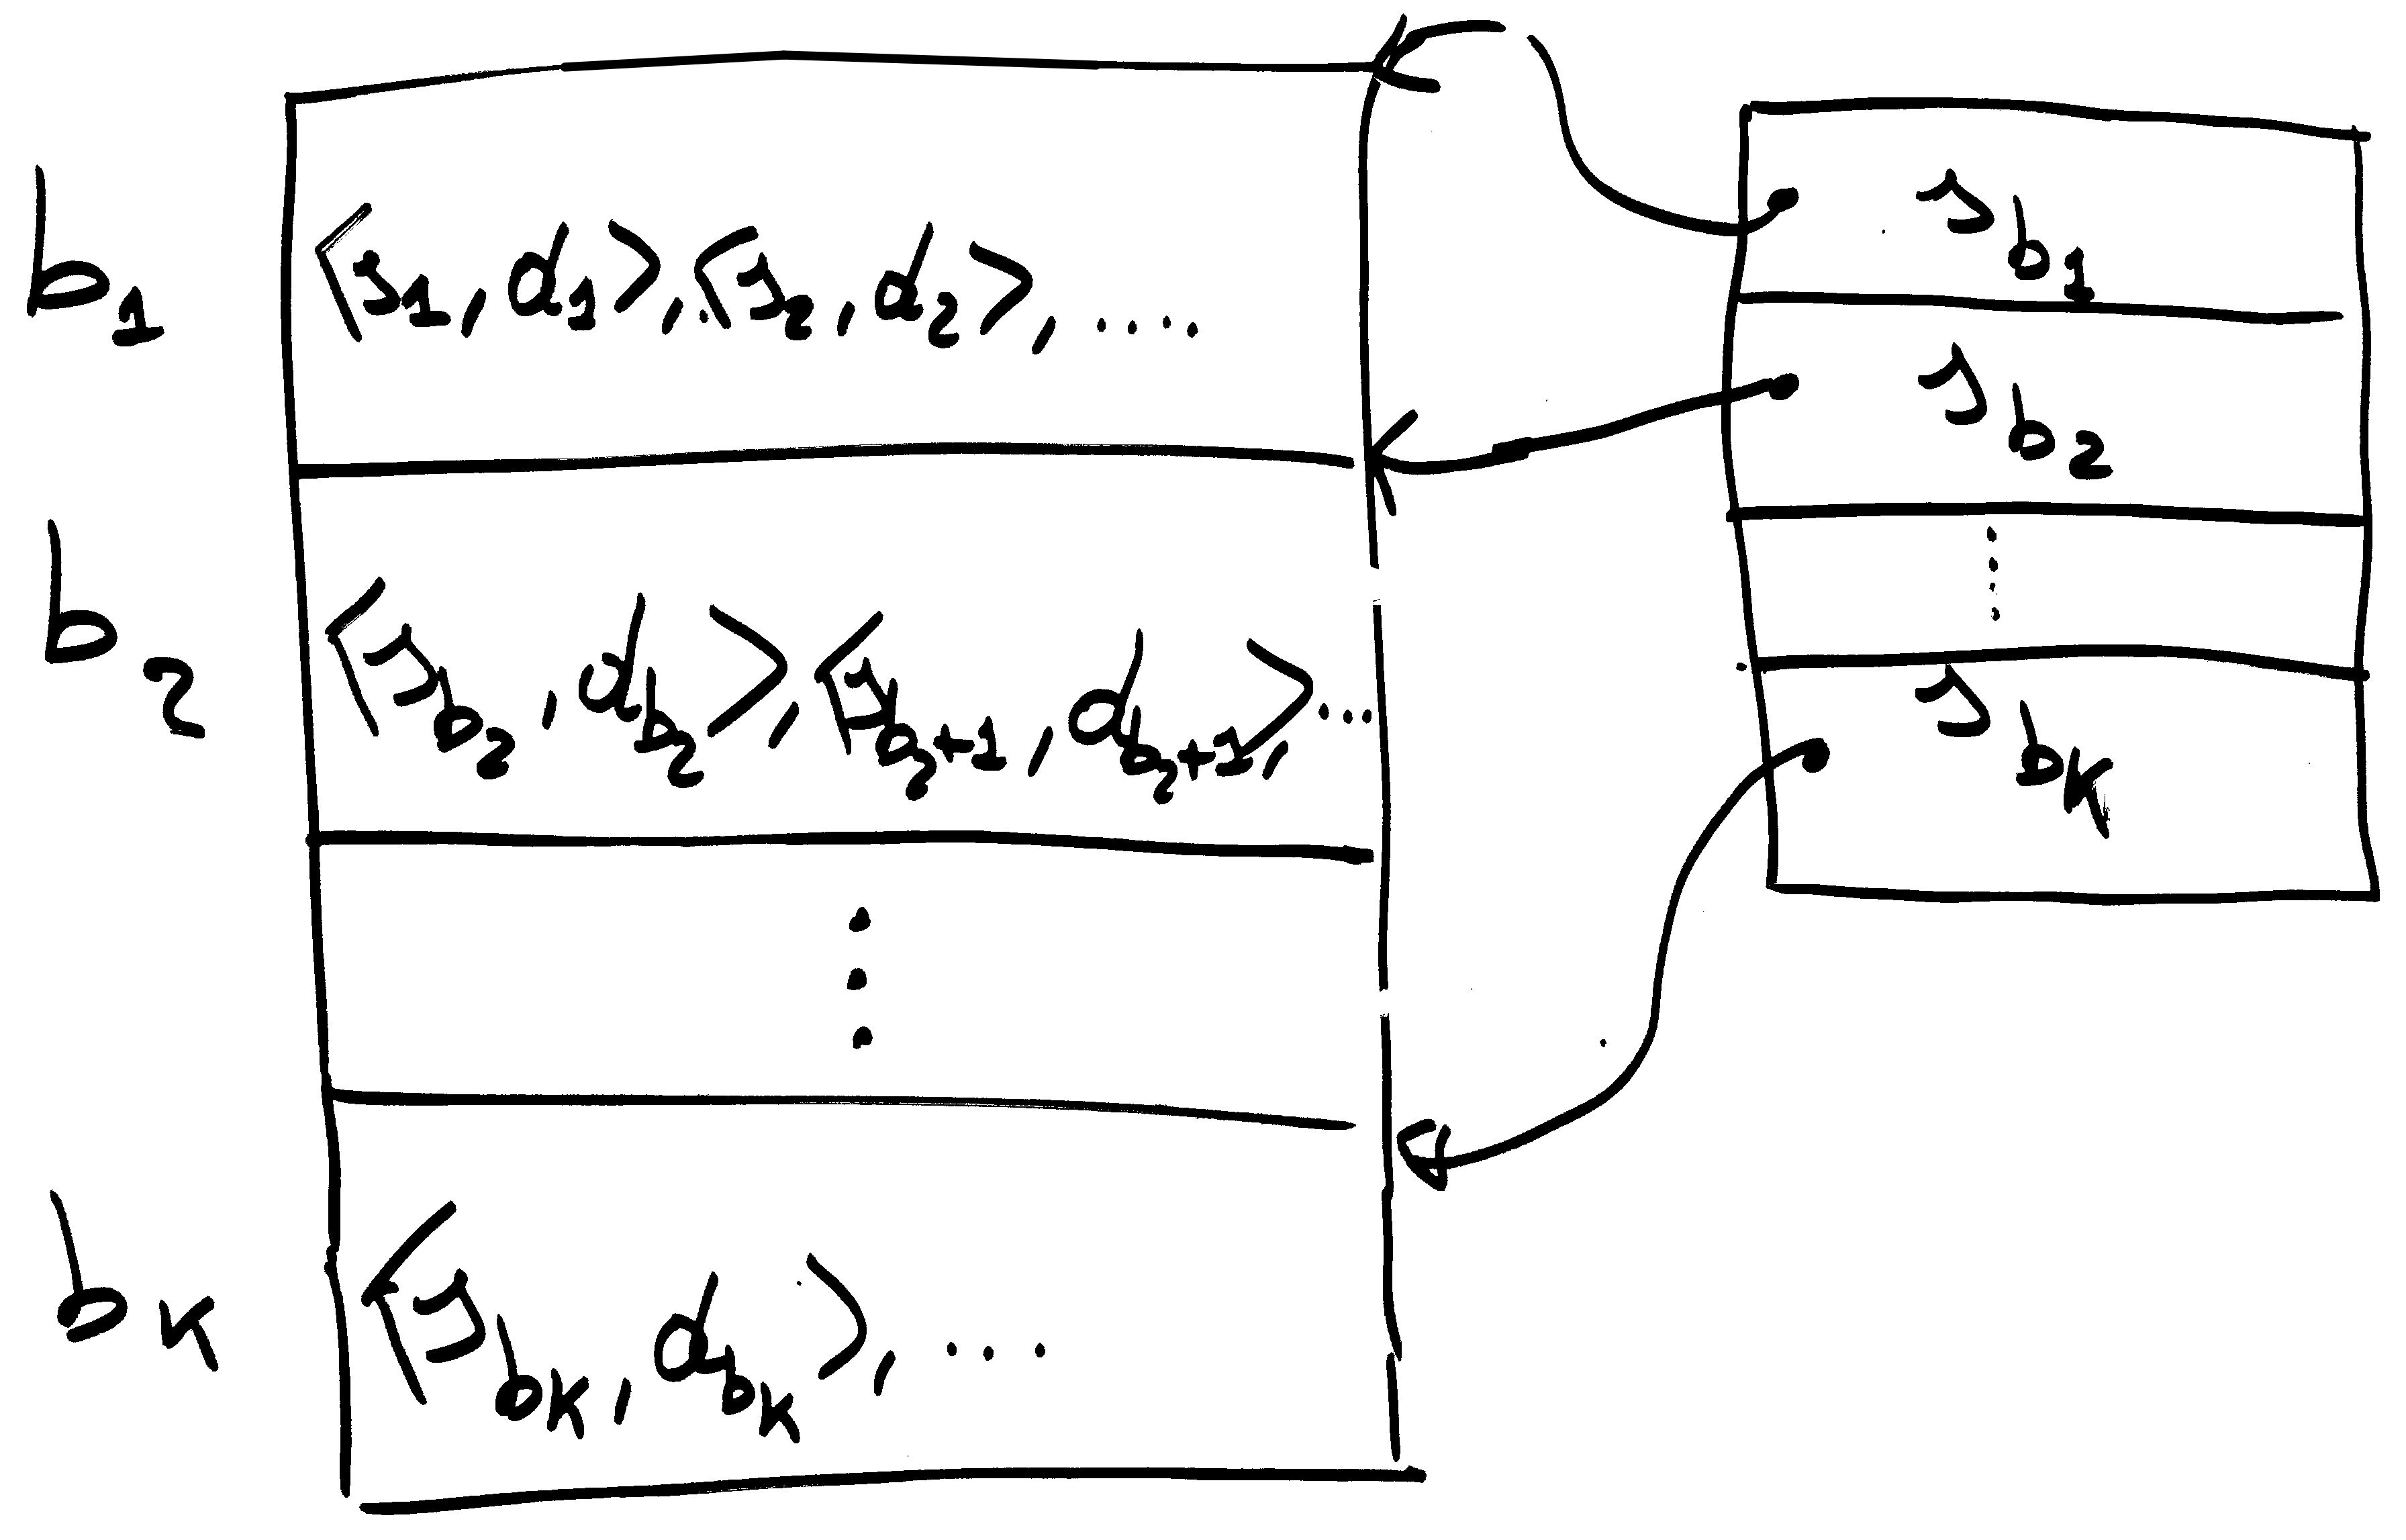
\includegraphics[width=0.6\linewidth]{assets/disk_map_base}
	\caption[]{Data organization}
	\label{fig:diskmapbase}
\end{figure}

In the real implementation, the pages' term heads $s_{b_i}$ are only stored in the look-up table, the data $d_i$ are compressed using \textit{variable bytes} and the other strings $s_j$ are compressed by cutting the common prefix they've with the page's head, so a generic key-value pair is more like:
$\left<	\left< p(s_{b_i}, s_j), {s'}_j \right>, c(d_j)	\right>$; where $p()$ is the length of the common prefix, $ {s'}_j$ is the string without the common prefix, and $c(d_j)$ is the compressed datum. The prefix's length is stored on a eight bit unsigned number, thus allowing for a maximum term's length of 255 bytes.

\paragraph{Complexity}
For simplicity's sake our implementation makes use of binary search to find in which page a term is stored and a linear scan to find it in the page, giving us a time complexity of 
$O\left(	|T|\cdot\log(k) + m	\right)$,
a space complexity, with regard to system memory, of
$O\left(	|T|\cdot k	\right)$
--- since we only have to keep the heads in memory --- and an I/O complexity of
$O\left(	1	\right)$, assuming all pages' heads fit in memory.

\subsection{Data}

\paragraph{Local lexica}
Each local lexicon stores the terms' information as \texttt{LexiconValue} during the first pass and then as \texttt{SigmaLexiconValue} in the second pass, when the upper bounds are computed and the skipping lists built.

Both structures store the number of docs in which such term appears and pointers to the compressed term frequencies and documents' ids. The latter structure also contains the skipping list and the upper bounds for \textit{TFIDF} and \textit{BM25}.

\paragraph{Global lexicon}
The only global lexicon just stores the total number of documents each term appear in, this is necessary to correctly compute the \textit{IDF} term.



\chapter{Query processing}


\chapter{Benchmarks}


\section{TREC evaluation}

\paragraph{}
To assess the system's performance, we utilized the TREC Eval tool, which was created by the Text REtrieval Conference (TREC) to establish a standardized method for comparing the efficacy of various search engines.

TREC Eval accepts a collection of search outcomes and relevant documents as input, subsequently employing several evaluation metrics to gauge the search result quality. These metrics encompass reciprocal rank, alongside more sophisticated measures such as mean average precision (MAP) and normalized discounted cumulative gain (NDCG).

\paragraph{Results}
The following table \ref{tab:metric_comparison} makes comparisons of our engine's performance with other search engines freely available, we used the  \href{https://msmarco.blob.core.windows.net/msmarcoranking/msmarco-test2020-queries.tsv.gz}{\texttt{msmarco-test2020-queries}} and set those engines to retrieve the first twenty results for each query.

\begin{table}[H]
	\centering
	\begin{tabular}{|l|>{\ttfamily}r|>{\ttfamily}r|>{\ttfamily}r|}
		\hline
		Metric & \normalfont\textbf{Ours} & \normalfont\textbf{Anserini} & \normalfont\textbf{Chang's} \\
		\hline
		mAP & 0.1982 & 0.1942 & 0.0794 \\
		RR & 0.8110 & 0.8215 & 0.7285 \\
		ndcg & 0.3376 & 0.3364 & 0.1681\\
		ndcg@10 & 0.4750 & 0.4876 & 0.4075 \\
		ndcg@20 & 0.4705 & 0.4705 & - \\
		set P & 0.4815 & 0.4667  & 0.5163 \\
		set R & 0.2600 & 0.2496 & 0.0987 \\
		set F & 0.2781 & 0.2670 & 0.1437 \\
		\hline
	\end{tabular}
	\caption{comparison of our project and Anserini's}
	\label{tab:metric_comparison}
\end{table}

\section{Time statistics}

\paragraph{}
The table presents the query processing times for the provided collection. 

Furthermore, we have included a histogram illustrating the distribution of execution times for run queries, comparing two methods: BMM and DAAT. This graphical representation allows for a visual comparison of the execution time distribution between the two query processing approaches.

\subsection{Queries' execution times}
	\begin{table}[h]
		\centering
		\begin{tabular}{|l|>{\ttfamily}r|>{\ttfamily}r|>{\ttfamily}r|}
			\hline
			Algorithm & \normalfont\textbf{AVG [ms]} & \normalfont\textbf{STD DEV [ms]} & \normalfont\textbf{MAX [ms]} \\
			\hline
			DAAT & 25.88 & 19.69 & 78.68 \\
			BMM & 6.67 & 6.29 & 42.48 \\
			\hline
		\end{tabular}
		\caption{Execution times in milliseconds for different algorithms}
		\label{tab:algorithm_times}
	\end{table}
	
	\begin{figure}[H]
		\centering
		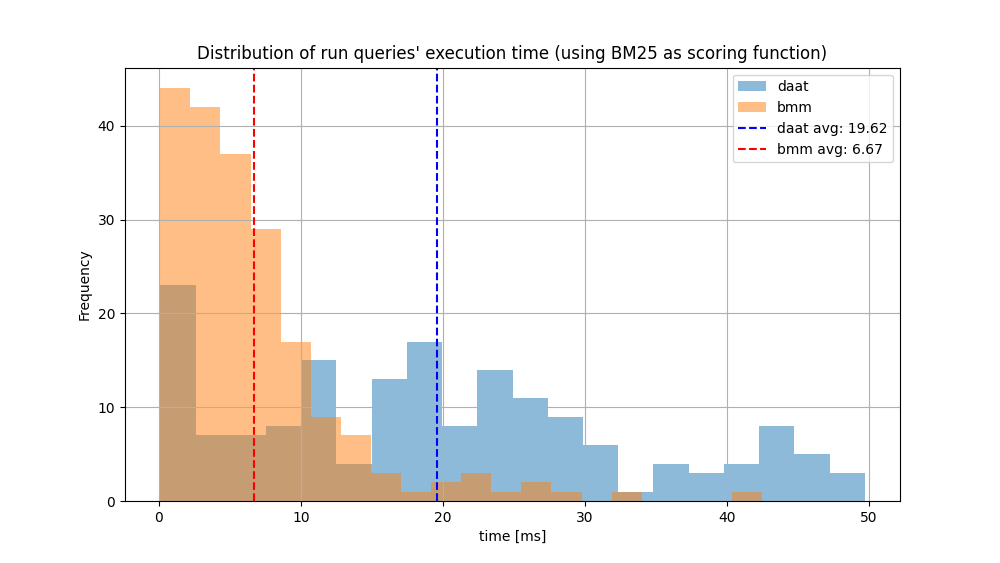
\includegraphics[width=1\textwidth]{assets/times_distrib.png}
		\caption{Distribution of times}
		\label{fig:time_distribution}
	\end{figure}
	
\subsection{Index's construction time}
\lstinputlisting[caption={Indexing program's output: it takes less than 1 minute and 20 seconds to build it}, label={lst:example_output}]{assets/build time.txt}
	
\section{Files' size}

\paragraph{}
The following table shows the file sizes presented in megabytes, divided int the indices' main files: Document Index, Local Lexicon, and Posting List.

\begin{table}[H]
	\centering
	\begin{tabular}{|l|*{5}{c|}c|}
		\hline
		& \textbf{Partition 0} & \textbf{Partition 1} & \textbf{Partition 2} & \textbf{Partition 3} & \textbf{Partition 4} & \textbf{Total} \\
		\hline
		Document Index & 46 & 47 & 46 & 46 & 17 & \textbf{202} \\
		Local Lexicon & 22 & 23 & 23 & 23 & 12 & \textbf{103} \\
		Posting Lists & 131.5 & 174.5 & 174.5 & 173.5 & 61.7 & \textbf{715.7} \\
		\hline
		\multicolumn{6}{|c|}{Global Lexicon} & \textbf{14} \\
		\hline
		\multicolumn{6}{|c|}{\textbf{TOTAL}} & \textbf{1034.7} \\
		\hline
	\end{tabular}
	\caption{Files' sizes, figures in megabytes}
	\label{tab:spanning_table}
\end{table}

\paragraph{}
To provide a clearer visualization, we have included a tree diagram below where the files' structure is depicted.

\lstinputlisting[caption={Files tree}, label={lst:tree}]{assets/files sizes.txt}


\end{document}          
